%------------------------------------------------------------------
% Preamble: provides useful commands and default settings
%------------------------------------------------------------------
%==================================================
% Standard
%==================================================
\documentclass[11pt]{article} % Page setup
\usepackage[top=1in, bottom=1in, left=1in, right=1in]{geometry} % Margin setup
\usepackage[square,sort,comma,numbers]{natbib}  % Reference Formatting
\usepackage{fancyhdr} % Header setup
\usepackage[toc,page]{appendix}
\usepackage[hang,flushmargin]{footmisc}
\usepackage{textpos}

%==================================================
%Typesetting Packages
%==================================================
\usepackage[colorlinks=true,linkcolor=Blue,citecolor=Red,urlcolor=Blue]{hyperref} % sets the color of hyperlinks
\usepackage{url} %Allows urls to be displayed properly
\usepackage{amsmath,amssymb} % Highly recommended as an adjunct to serious mathematical typesetting; amssymb provides extended symbol collection
\usepackage{textcomp} % Package supports Text Companion fonts (baht, bullet, copyright, musicalnote, onequarter, section, and yen)
\usepackage{color} % Provides foreground (text, rules, etc.) and background color management
\usepackage{colordvi} % Allows for using named colors when typsetting output
\usepackage[usenames,dvipsnames,svgnames,table]{xcolor} % Extends the color package; several color tints, shades, tones, and mixes of arbitrary colors
\definecolor{arsenic}{rgb}{0.23, 0.27, 0.29}
\definecolor{color18}{rgb}{0.5,0.5,0.5} % Defines a color named "color18"
\usepackage{bm} % bold math
\usepackage{siunitx} % si units package 
\newcommand{\SIper}{\SI[per-mode=symbol]} % Special command for the SI unit package
\usepackage{enumerate} % Allows for the enumerate style to be changed 
%\usepackage{enumitem}
\usepackage{alphalph}
\usepackage{setspace}
\usepackage{blindtext}
\usepackage{soul}
\usepackage[tocindentauto]{tocstyle}
\usepackage{algorithm}
\usepackage{algpseudocode}
\usepackage{multirow}
\usepackage{mathtools}
\usepackage{minted}
\usepackage{afterpage}
\usepackage{float}
\usepackage{changepage}
\numberwithin{equation}{section}
%\usepackage{mathptmx}

% ==================================================
%Figure packages
% ==================================================
\usepackage{graphicx} % Include figure files
\usepackage{rotating} % Performs all rotations including complete figures and tables with their captions ON ONE PAGE
\usepackage{lscape} % Rotates the page contents but not the page number; can be applied across many pages
\usepackage[font=scriptsize,format=plain,labelfont=bf]{caption} % Caption customization (also for tables)
\usepackage{subcaption} % Provides support for subcaptions
\usepackage{float} % Improved interface for defining float objects (figures and tables)
\usepackage{wrapfig} % Allows figures or tables to have text wrapped around them
\setlength{\parskip}{5pt} %Space between paragraphs
\setlength{\parindent}{0pt} %Paragraph Indent size
\usepackage{fancybox}
\usepackage{mdframed}
\usepackage{makeidx}
\usepackage{tablefootnote}

% ==================================================
% Table packages
% ==================================================
\usepackage{longtable} % allow multipage tables
\usepackage{multicol}
\usepackage{multirow} % create tabular cells spanning multiple rows
\usepackage{dcolumn} % Align table columns on decimal point
\usepackage{threeparttable}
\usepackage{lipsum,booktabs}

% ==================================================
% Section Formatting 
% ==================================================
\usepackage{sectsty}
\allsectionsfont{\bfseries} %Sets ALL section font

%Title, author, date formats	
	\newcommand{\mytitle}[1]{\title{\bf{\textsf{#1}}}}
	\newcommand{\myauthor}[1]{\author{\textsf{#1}}}
	\newcommand{\mydate}[1]{\textsf{\date{#1}}}
	\newcommand{\mytoday}{\textsf{\today}}

%Section header formats	(Numbered)
	\newcommand{\mysection}[2]{\vspace{-5px}\section{#1}\label{#2}\vspace{-10px}}
	\newcommand{\myssection}[2]{\vspace{-5px}\subsection{#1}\label{#2}\vspace{-5px}}
	\newcommand{\mysssection}[2]{\vspace{-5px}\subsubsection{#1}\label{#2}\vspace{-5px}}

%Section header formats	(Unnumbered)	
	\newcommand{\mysectionN}[2]{\vspace{-5px}\section*{#1}\label{#2}\vspace{-10px}}
	\newcommand{\mysectionnonum}[2]{\vspace{-5px}\section*{#1}\label{#2}\vspace{-10px}}
	\newcommand{\myssectionN}[2]{\vspace{-5px}\subsection*{#1}\label{#2}\vspace{-5px}}
	\newcommand{\myssectionnonum}[2]{\vspace{-5px}\subsection*{#1}\label{#2}\vspace{-5px}}
	\newcommand{\mysssectionN}[2]{\vspace{-5px}\subsubsection*{#1}\label{#2}\vspace{-5px}}
	\newcommand{\mysssectionnonum}[2]{\vspace{-5px}\subsubsection*{#1}\label{#2}\vspace{-5px}}

%Paragraph header formats		
	\newcommand{\mypart}[2]{\part{#1}}
	\newcommand{\mypara}[2]{\paragraph{#1}}
	\newcommand{\myparaN}[2]{\paragraph*{#1}}
	\newcommand{\myparanonum}[2]{\paragraph*{#1}}

%References, etc.	
	\newcommand{\myref}[2]{\hyperref[#2]{#1~\ref{#2}}}
	\newcommand{\myrefexp}[3]{\hyperref[#3]{{#1}~{#2}}}
	\newcommand{\hilight}[1]{\colorbox{yellow}{#1}}
	\newcommand{\myfilename}[1]{\texttt{\textsf{#1}}}
	\newcommand{\mywebsite}[1]{\myfilename{\bf #1}}
	\newcommand{\commandline}[1]{\texttt{> #1}}
	\newcommand{\plusplus}[1]{#1{}\texttt{++}}

%Callout Box Creator	
	\newcommand{\callout}[3]
	{
	\begin{wrapfigure}{#1}{#2\textwidth}
	\vspace{-20pt}
	\centering
	\fbox{\parbox{#2\textwidth}{#3}}
	\vspace{-10pt}
	\end{wrapfigure}
	}

% ==================================================
% Track changes and commenting packages/commands
% ==================================================
\usepackage{todonotes}
	\newcommand{\sn}[1]{\todo[color=magenta!40,caption={}]{#1}}
	
\usepackage{comment}


	%Other colors available 
	%cyan
	%green
	%white
	%darkgray
	%brown
	%olive
	%pink
	%purple
	%violet


\usepackage{verbatimbox}
\usepackage{wrapfig} 
\usepackage{rotating}
\usepackage{mathrsfs}
\usepackage{cancel}
\usepackage{pdfpages}
\newcommand{\bs}{\boldsymbol}
\newcommand{\kpar}{k_{\shortparallel}}
\newcommand{\chebint}{\pmb{\mathscr{I}}}
\newcommand{\chebdiff}{\pmb{\mathscr{D}}}
\newcommand{\overbar}[1]{\mkern 1.5mu\overline{\mkern-1.5mu#1\mkern-1.5mu}\mkern 1.5mu}

%---------
% Beginning of document
%------------------------------------------------------------------
\begin{document}
\setcounter{secnumdepth}{5}
\setcounter{tocdepth}{4}

% Your Name
\begin{textblock*}{8cm}(15cm,-1cm)
	\noindent {Sachin Natesh} 
\end{textblock*}

\mysection{Immersed Boundary method for Poisson Equation}{}
Consider Poisson's equation,
\begin{align}
\displaystyle \nabla^2 \phi &= -\rho, \label{poisson}
\end{align}
on a triply periodic domain $\Omega := (x,y,z) \in[-L,L]^3$ subject to periodic boundary conditions. Here, $\phi$ is the electric potential and $\rho$ is the charge distribution given by
\begin{equation}
\rho(\bs x) = \displaystyle \sum_{k=1}^M q_k\Delta_q(\bs x - \bs y_k),
\end{equation}
for charges $q_k$ with positions $\bs y_k$, and $\Delta_q$ a spreading kernel. The electric field induced by the charge distribution is given by
\begin{equation}
\bs E = -\nabla \phi,
\end{equation}
and any function $\bs f(\phi,\bs x)$ can be evaluated at the charge locations with
\begin{equation}\label{interp}
\bs f(\phi,\bs y_k) =  \displaystyle \int_{\Omega} \bs f(\phi,\bs x)\Delta_q(\bs x - \bs y_k) d\bs x.
\end{equation}
\myssection{Spectral solver}{}
Taking the Fourier transform of $\myref{Eq.}{poisson}$ in $x,y$ and $z$ gives a trivial way to solve for $\phi$;
\begin{equation}\label{specsolve}
\hat{\phi}(\bs k) = \frac{\hat{\rho}(\bs k)}{||\bs k||^2},
\end{equation}
where $\bs k = \begin{pmatrix} k_x & k_y & k_z\end{pmatrix}$ is the vector of wave numbers in $x,y,z$, and $||\cdot||$ is the 2-norm. Specifically, $k_x,k_y,k_z = \frac{2\pi j}{2L}$, $j = -\frac{N}{2},\cdots, \frac{N}{2}-1$, where $N$ is the number of points in each axis. Note, to ensure the net charge in the unit cell is 0, we set $\hat{\rho}(\bs 0) =0$ and only use \myref{Eq.}{specsolve} for $\bs k \neq 0$.
\myssection{Solver using the Fourier symbol of 7 point centered difference Laplace operator}{}
Now, consider the centered second derivative matrix $\bs D^2 = \displaystyle \frac{1}{h^2}(\bs N - 2\bs I + \bs N^{-1})$, where $\bs I$ is identity and $\bs N$ is the shift matrix
\begin{equation}
\bs N = \begin{pmatrix} 
0 & 1 & 0 & \cdots & 0 \\
0 & \ddots & \ddots & \ddots & \vdots \\
\vdots & & \ddots & \ddots & 0 \\
0 & & & 0 & 1 \\
1 & 0 & \cdots & \cdots & 0
\end{pmatrix}.
\end{equation}
Using the fact that the Fourier vectors $\bs v_k = \{e^{ilkh}\}_{l=0}^{N-1}$ for wave numbers $k$ are eigenvectors of $\bs N$ with eigenvalue $e^{ikh}$, we can diagonalize $\bs D^2 = \bs V^\star \bs \Lambda \bs V$ in the discrete Fourier basis $\bs V$, with the diagonal elements given by
\begin{equation}
(\bs \Lambda)_k = \displaystyle -\frac{4}{h^2}\sin^2\Big(\frac{kh}{2}\Big).
\end{equation}
Then, the Fourier symbol of the discrete centered difference Laplace operator $\bs D_x^2 + \bs D_y^2 + \bs D_z^2$ gives an alternate way to differentiate in Fourier space and solve \myref{Eq.}{poisson}:
\begin{equation}\label{diffsolve}
\hat{\phi}(\bs k) = \displaystyle \frac{\hat{\rho}(\bs k)}{\frac{4}{h^2}||\sin(\frac{\bs k h}{2})||^2}%\sin^2\Big(\frac{k_xh}{2}\Big) + \sin^2\Big(\frac{k_yh}{2}\Big) + \sin^2\Big(\frac{k_zh}{2}\Big) \Big)}.
\end{equation}
As in the spectral solver, to ensure the net charge in the unit cell is 0, we set $\hat{\rho}(\bs 0)=0$ and only use \myref{Eq.}{diffsolve} for $\bs k \neq 0$.
\myssection{Solver using the Fourier symbol of 24 point centered difference Laplace operator}{}
Using the same arguments as in the previous section, one can derive the Fourier symbol of a 4th order, 24 point approximation to the Laplacian. In this case, we solve for the potential in the Fourier domain with
\begin{equation}
\hat{\phi}(\bs k) = \displaystyle \frac{\hat{\rho}(\bs k)}{\frac{4}{6h^2}\big(\cos(\bs k h) \cdot \bs{1} + \cos(k_x h)\cos(k_y h) + \cos(k_x h) \cos(k_z h) + \cos(k_y h)\cos(k_z h) - 6 \big)}
\end{equation}
\mysection{Numerical experiments}{}
Suppose there are two charges of $+1,-1$ with random positions $\bs y_1,\bs y_2$ within $L/2$ in each direction. We solve for $\phi$ given this configuration, resample the positions, and repeat the process many times. Note, this setup tests both rotational and translational invariance, since we're only fixing the distance between charges before the trials. For each 2nd order solve, we compute the electric field using the Fourier symbol of the centered first derivative operator $\bs D^1 = \displaystyle \frac{1}{2h}(\bs N - \bs N^{-1})$ as
\begin{equation}
\hat{\bs E}_{\bs k} = -\frac{i}{h}\sin(\bs k h)\hat{\phi}(\bs k),
\end{equation}  
or, in the case of a 4th order solve,
\begin{equation}
\hat{\bs E}_{\bs k} = \displaystyle -\frac{i}{h}\Big(\frac{4}{3}\sin(\bs kh) - \frac{1}{6}\sin(2\bs kh)\Big)\hat{\phi}(\bs k).
\end{equation}
The field in real space is recovered through
\begin{equation}
\bs E = \bs V^{\star}_x \bs V^{\star}_y \bs V^{\star}_z \hat{\bs E}.
\end{equation}
We then use \myref{Eq.}{interp} to interpolate the electric field $\bs E$ at one of the charge locations resulting in a vector $\bs E_q$. The component of $\bs E_q$ pointing along $\hat{\bs r} = \displaystyle \frac{\bs y_2 - \bs y_1}{||\bs y_2-\bs y_1||} = \frac{\bs r}{r}$ is given by 
\begin{equation}
E_q(r) = \bs E_q \cdot \hat{\bs r},
\end{equation}
and the magnitude of the non-central component of the force is
\begin{equation}
\text{non-centrality} = \displaystyle \frac{||\bs E_q - E_q(r)\hat{\bs r}||}{E_q(r)}.
\end{equation}
In the following tests, we collect and analyze the statistics of $E_q(r)$ and non-centrality for several kernels. We also compare $E_q(r)$ obtained by the solver to the Coulomb field magnitude $1/(4\pi r^2)$. Lastly, we use the fact that Gaussian charge densities with width $\sigma$ result in 
\begin{equation}\label{egauss}
E_q^{\text{Gauss}}(r) = \displaystyle \frac{1}{4\pi} \Big(\frac{\text{erf}\big(\frac{r}{2\sigma}\big)}{r^2} - \frac{\exp(\frac{-r^2}{4\sigma^2})}{r\sigma \sqrt{\pi}}\Big)
\end{equation}
to compute effective Gaussian widths for non-Gaussian kernels. The domain is $[-L,L]^3$ with $L=32$ and $h=0.5$. All $\%$-errors are reported as 
\begin{equation}\label{pererr}
\text{\%-error} =\displaystyle  \frac{2\sigma_f}{\overbar{\bs f}}\times 100\%, 
\end{equation}
for data $\bs f$ with standard deviation $\sigma_f$ and some truth value $\overbar{\bs f}$.

\myssection{Full width Gaussian kernel}{}
First, we check the correctness of the implementation and post-processing when using a Gaussian kernel and the spectral method given by \myref{Eq.}{specsolve}. We know the analytical solution for this problem from \myref{Eq.}{egauss}. Then, the fitted $\sigma$ value for the Gaussian should match what we actually use, and convergence to the Coulomb law should be exponential. The results for $\sigma = 12h/8$, i.e. 12 points per $8\sigma$, are given in the following figure.
\begin{figure}[H]
	\centering
	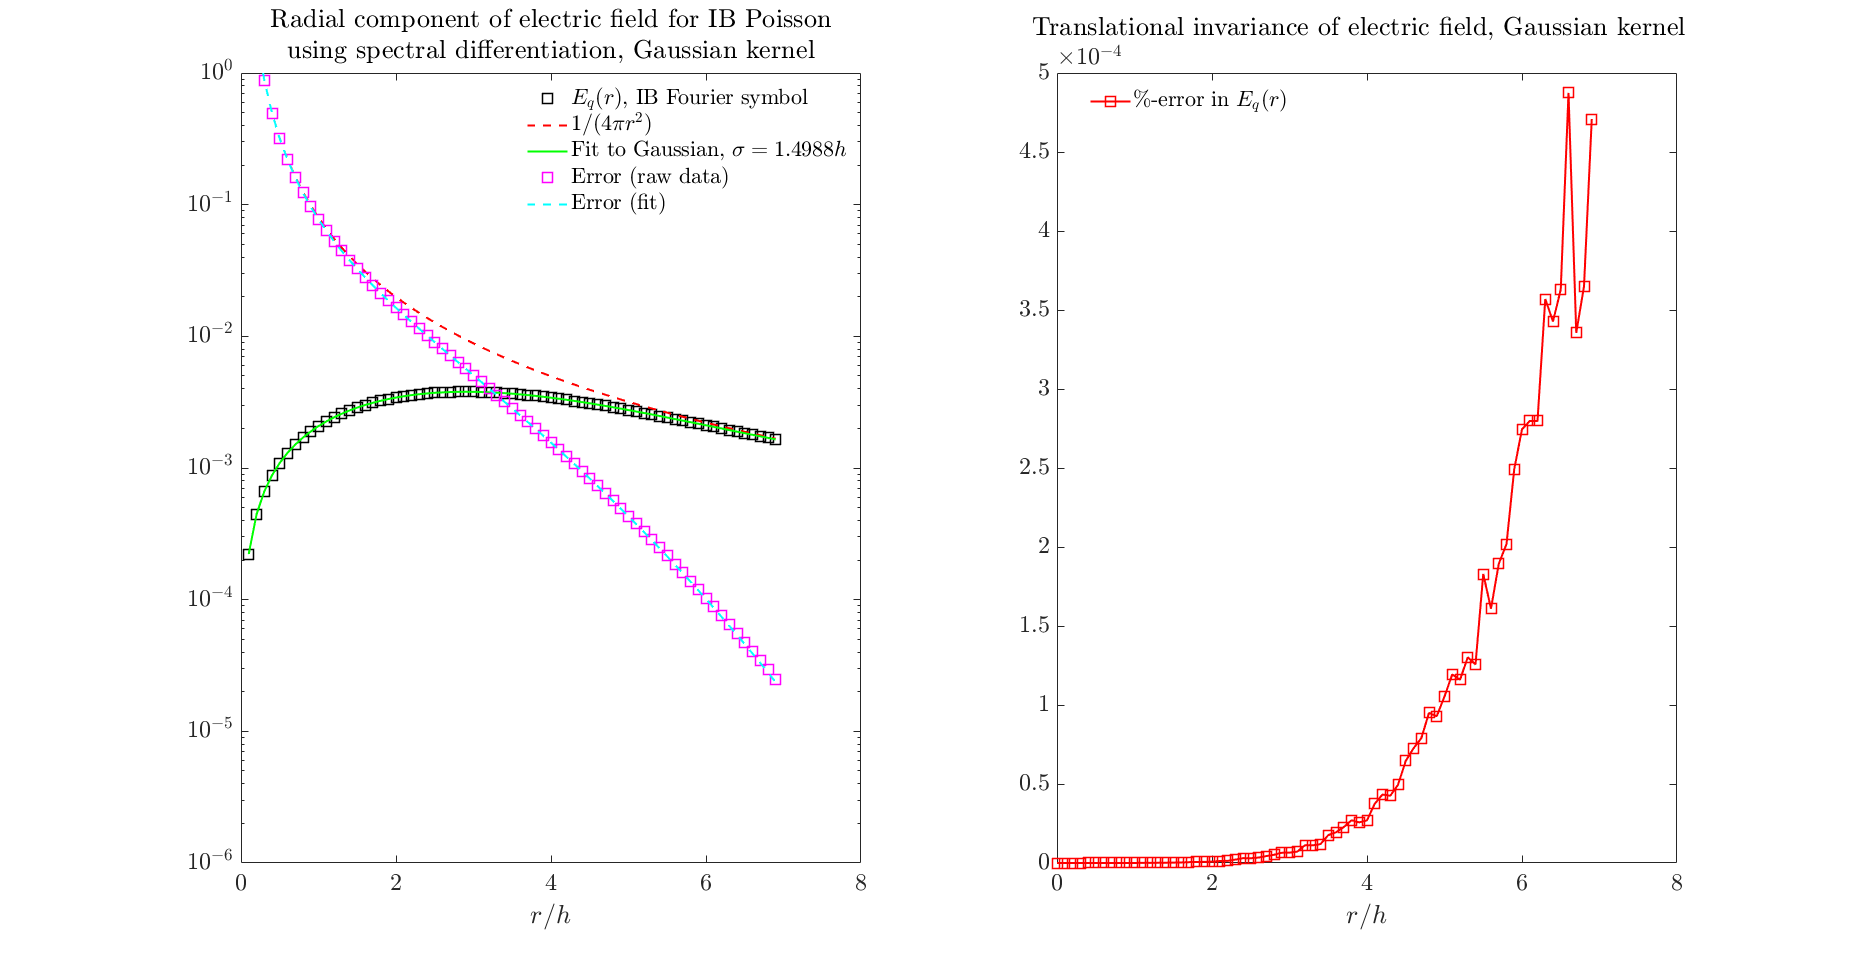
\includegraphics[width=1\columnwidth]{../Figures/Gaussian_L32_N128.png}
	\caption{Results for Gaussian kernel. Note, we use $\sigma/h = 1.5$, and the fitted value approximately agrees.}\label{gauss}
\end{figure}
\newpage
\myssection{Peskin kernels}{}
Here, we consider the $4,5$ and $6$ point Peskin kernels and compare results for the $4,6$ point kernels using our fast solver to those obtained using a multigrid IB method. Additionally, we compare the difference between 2nd and 4th order fast solvers with the $6$ point kernel.
\begin{figure}[H]
	\centering
	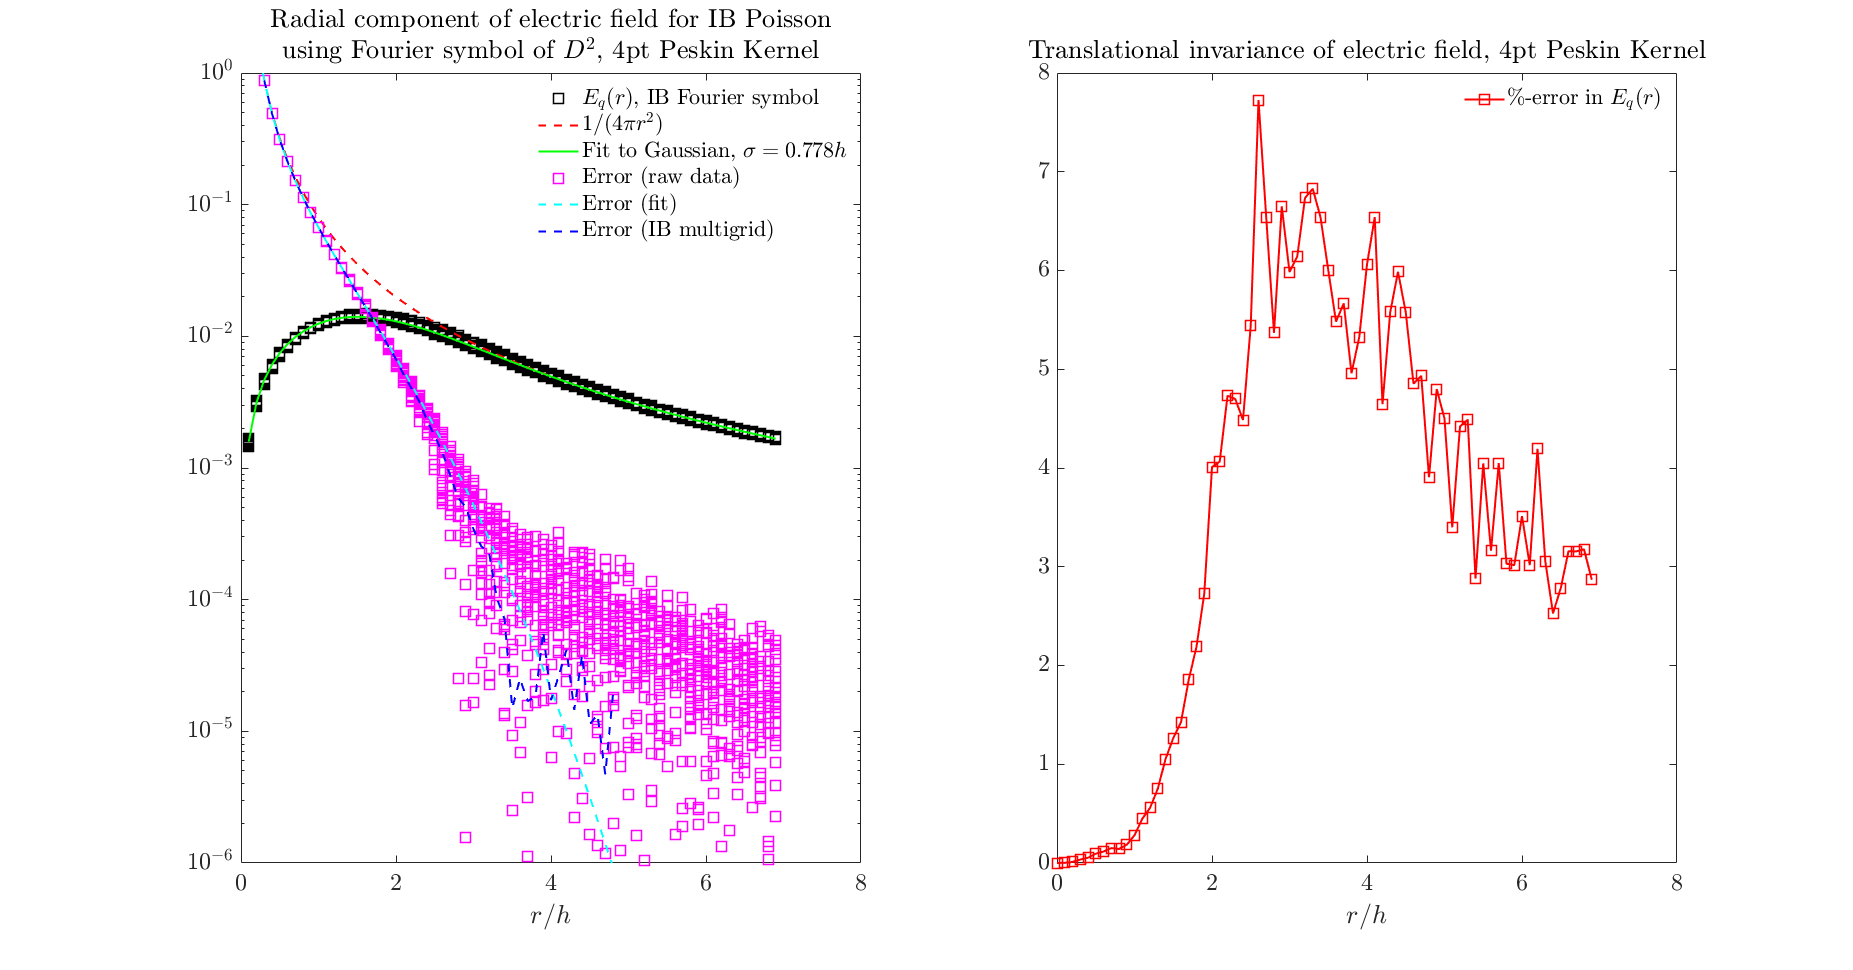
\includegraphics[width=1\columnwidth]{../Figures/4pt_peskin.png}
	\caption{Results for 4pt peskin kernel.}\label{pesk4}
\end{figure}
\begin{figure}[H]
	\centering
	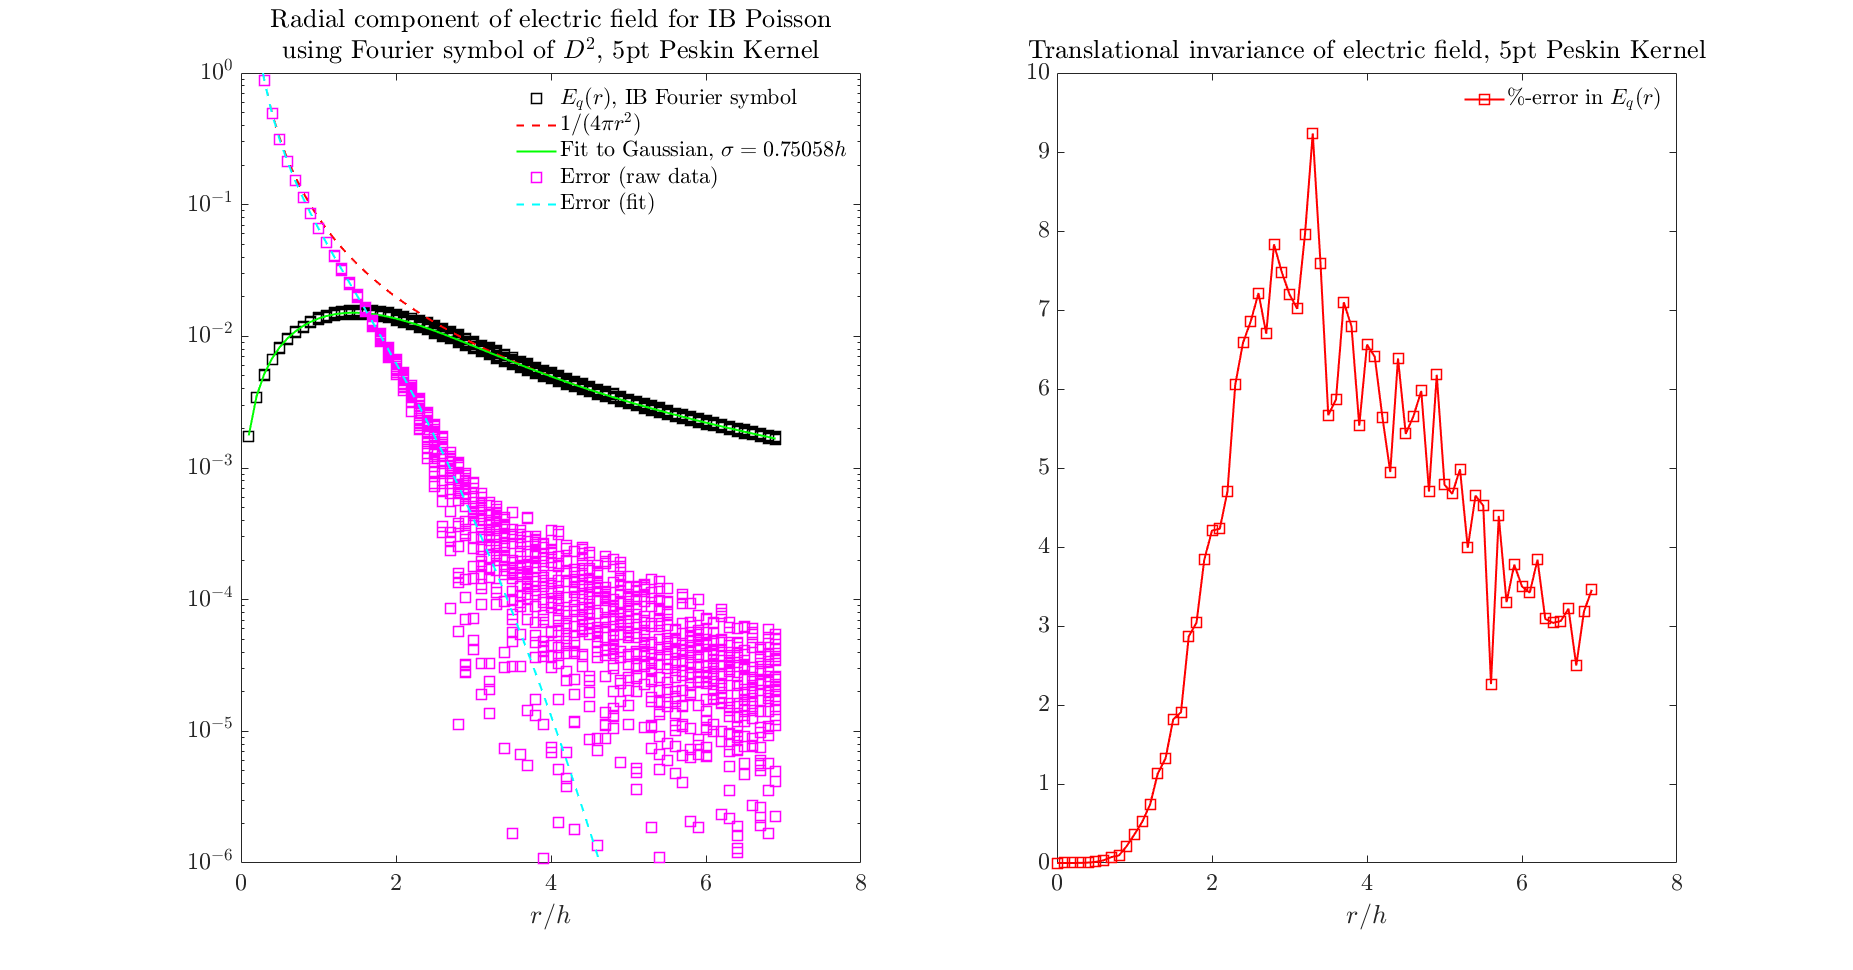
\includegraphics[width=1\columnwidth]{../Figures/5pt_peskin.png}
	\caption{Results for 5pt peskin kernel.}\label{pesk5}
\end{figure}
\begin{figure}[H]
	\centering
	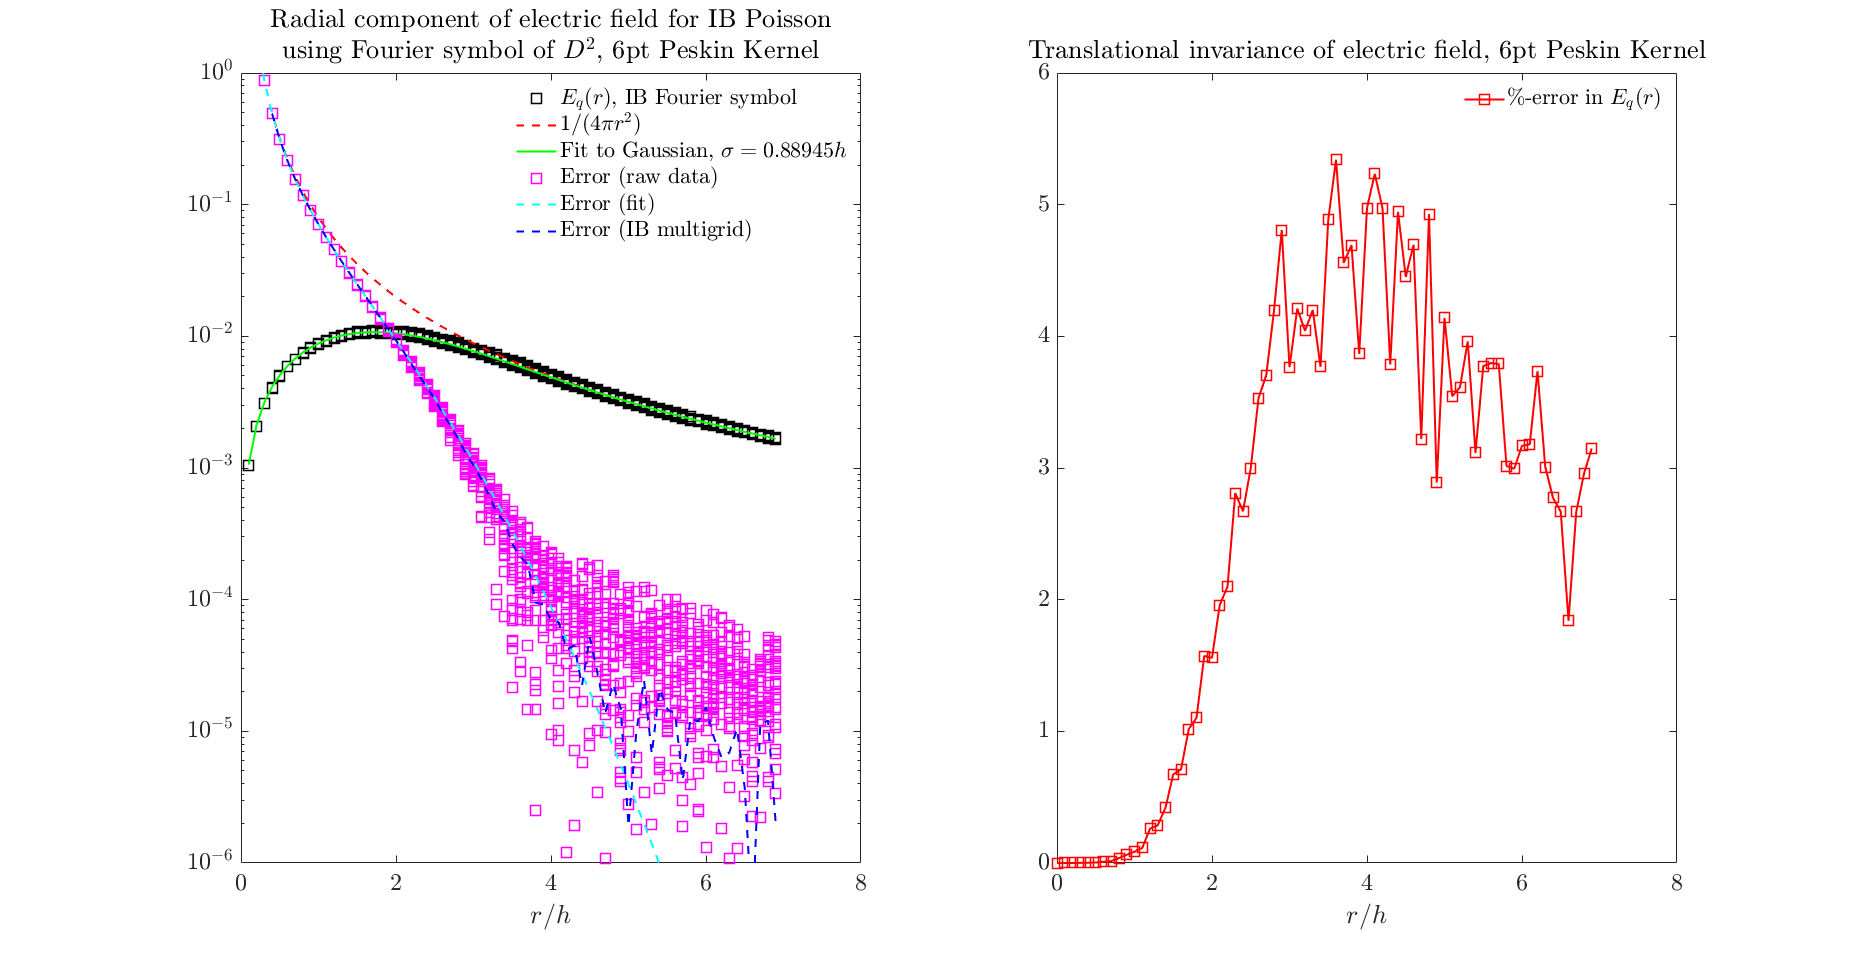
\includegraphics[width=1\columnwidth]{../Figures/6pt_peskin.png}
	\caption{Results for 6pt peskin kernel.}\label{pesk6}
\end{figure}
\begin{figure}[H]
	\centering
	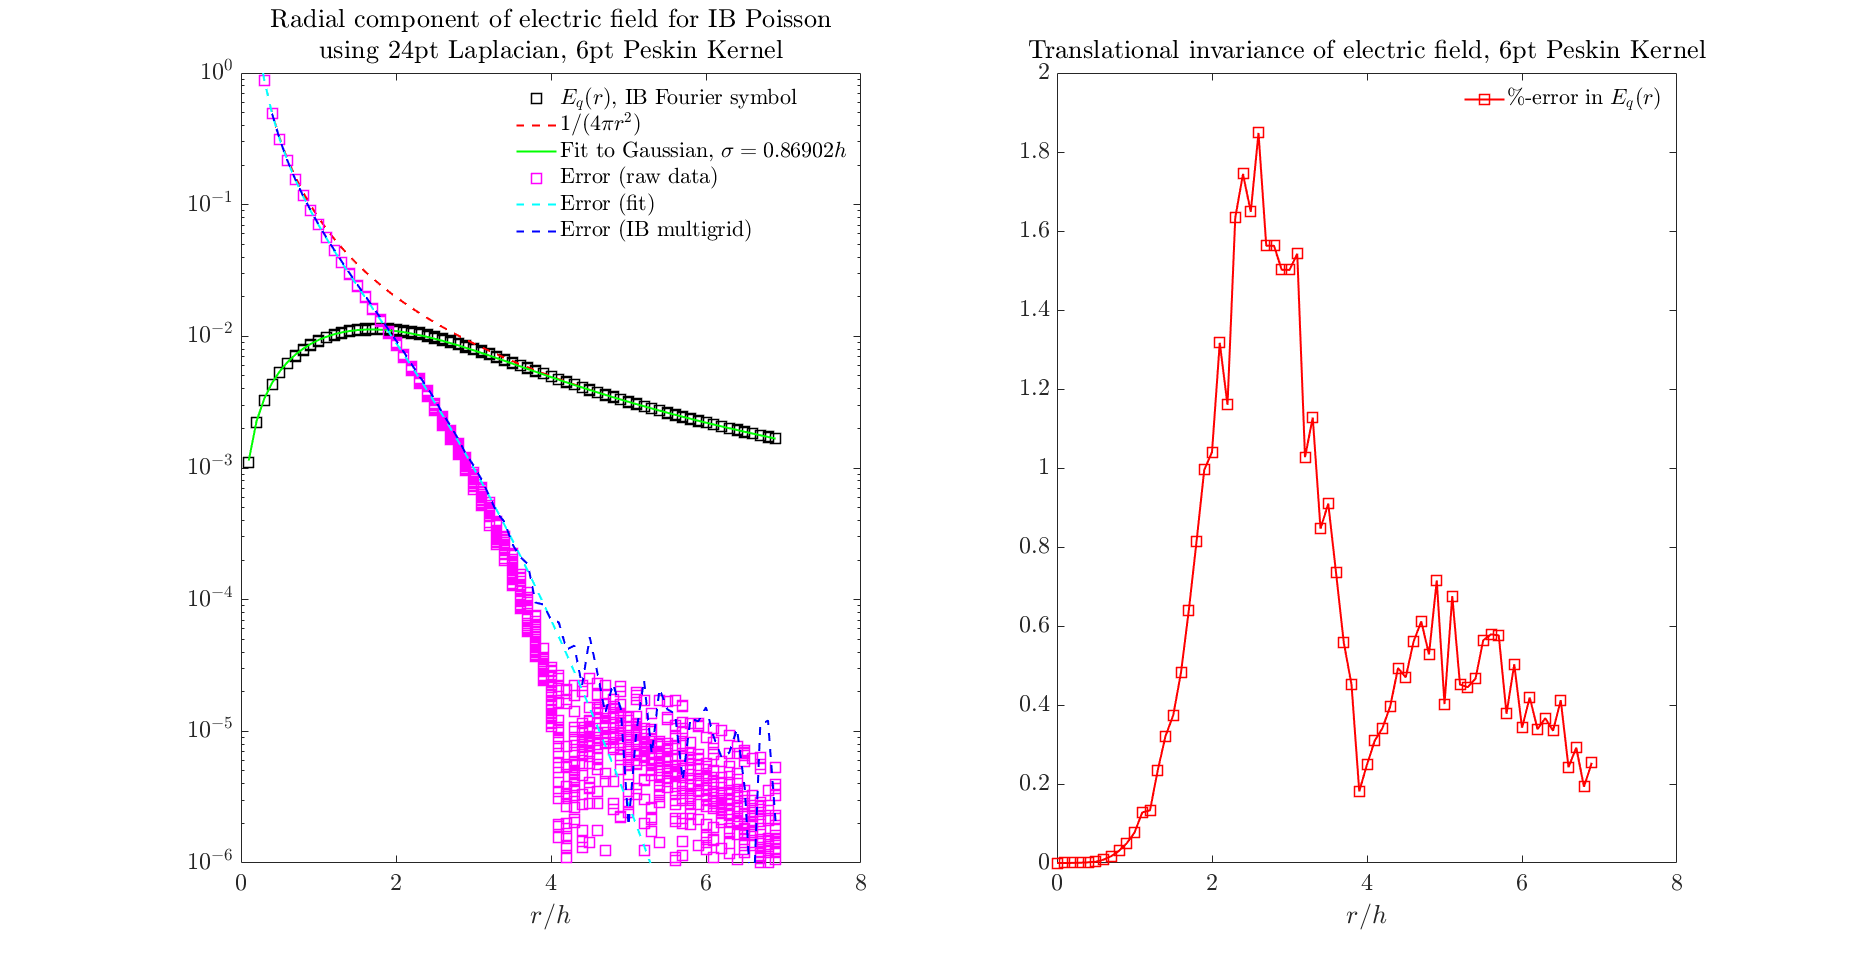
\includegraphics[width=1\columnwidth]{../Figures/6pt_peskin_24ptlap_correct.png}
	\caption{Results for 6pt peskin kernel using a 24pt Laplacian. As expected, we have better translational invariance than the 2nd order solve, and gain around 1 digit of accuracy in the Coulomb field.}\label{pesk624pt}
\end{figure}
\newpage
In order to more clearly see the difference in the rate of convergence to the Coulomb field between the 2nd and 4th order solvers for the 6 point kernel, we modify the selection of charge configurations as follows. First, we pick $\bs y_1$ uniformly at random. The position of the second charge is $\bs y_2 = \bs y_1 \pm \displaystyle \frac{sL}{8}$ for some $s \in [0,1]$. Then, we translate this diagonal configuration diagonally by $\frac{LU(0,1)}{4}$, solve, and repeat many times. In this way, we are only checking diagonal translational invariance for a diagonal charge configuration. The result is shown in the following figure.

\begin{figure}[H]
	\centering
	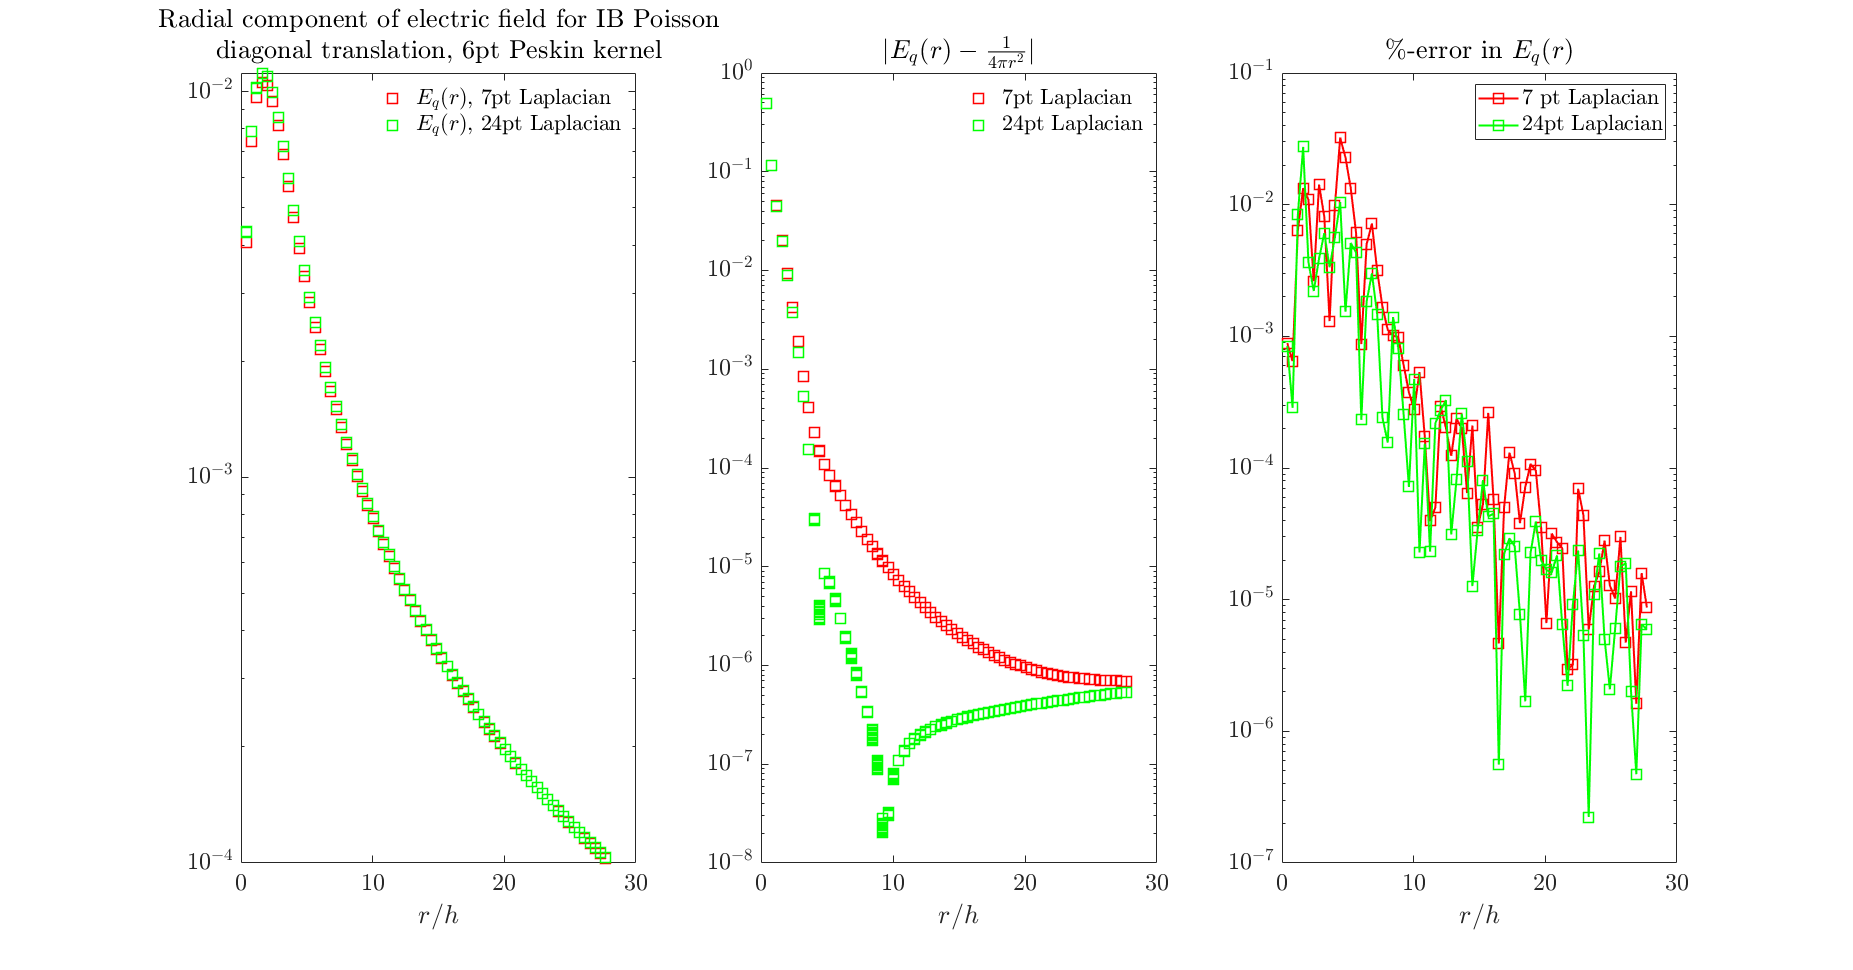
\includegraphics[width=1\columnwidth]{../Figures/6pt_peskin_24ptlap_diag_compare.png}
	\caption{Comparing results for 6pt peskin kernel using a 7pt or 24pt Laplacian with diagonal translation. The difference in the algebraic decay of the error w.r.t the Coulomb law between the two solvers is clear, and we note that the translational invariance decays for this diagonal orientation and translation. The eventual increase in the error for the 24pt Laplacian is likely due to dominance of periodic artifacts at larger separations.}\label{pesk624pt}
\end{figure}


\newpage
\myssection{ES kernel}{}
For reference, the ES kernel is given by 
\begin{equation}
\phi_{\beta}(z;\alpha) = \displaystyle \frac{1}{\displaystyle \int_{-\alpha}^\alpha e^{\beta(\sqrt{1-(\frac{z}{\alpha})^2}-1)}dz} \begin{cases}
e^{\beta(\sqrt{1-(\frac{z}{\alpha})^2}-1)},\quad &|\frac{z}{\alpha}| \leq 1\\
0,\quad &\text{otherwise},
\end{cases}
\end{equation}
where $\alpha = wh/2$, $w$ is the number of points to which we spread in each direction, and we've normalized the kernel so that integrating it over its support gives 1. We want to use the optimal ES kernel with $w=6$ in the sense of minimizing translational invariance. To this end, we consider a single charge with location selected uniformly at random in a cube of width $h_{xy}$ at the center of the grid. For several $\beta$s and charge locations, we evaluate the potential on the charge and ultimately measure how the potential changes with translation using \myref{Eq.}{pererr}. 

\begin{figure}[H]
	\centering
	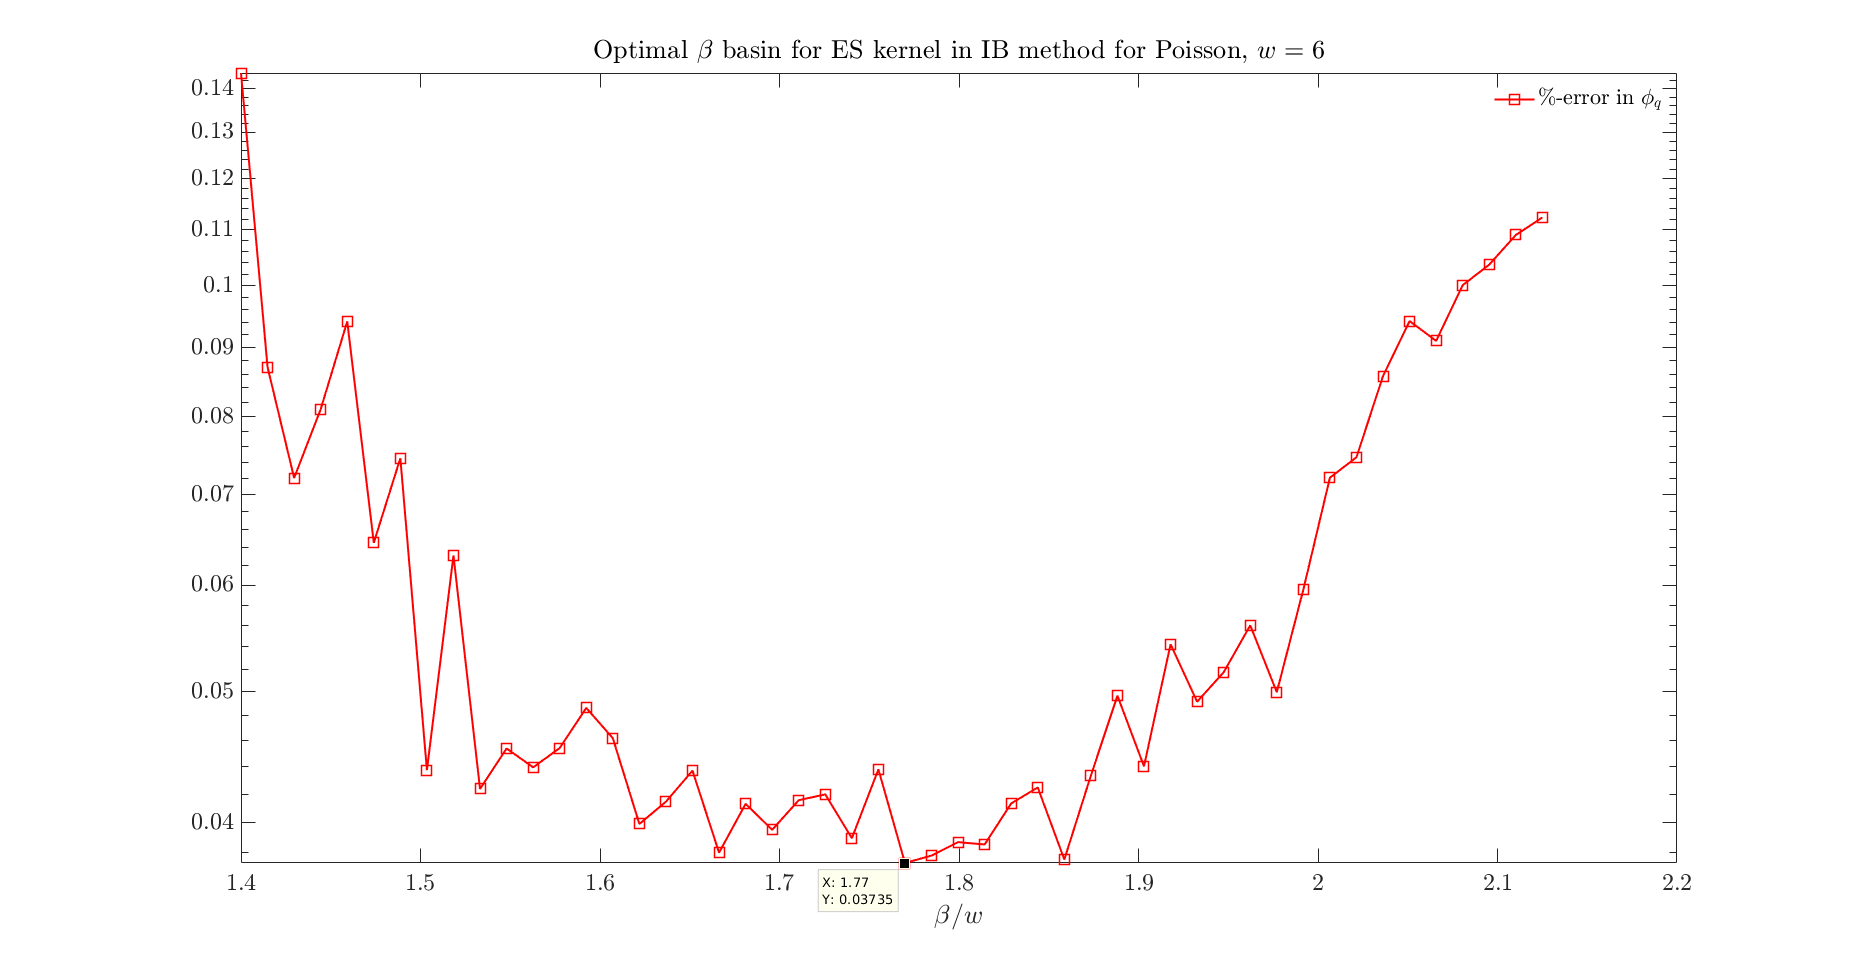
\includegraphics[width=1\columnwidth]{../Figures/6pt_ES_opt_beta.png}
	\caption{Optimal $\beta$ basin to minimize translational invariance for ES kernel using $w=6$. We see that $\beta/w \approx 1.77$ gives the minimal percent error.}\label{ESopt}
\end{figure}
Now, we run the same tests as in the previous section for $\beta/w = 1.55, 1.7, 1.85$.
\begin{figure}[H]
	\centering
	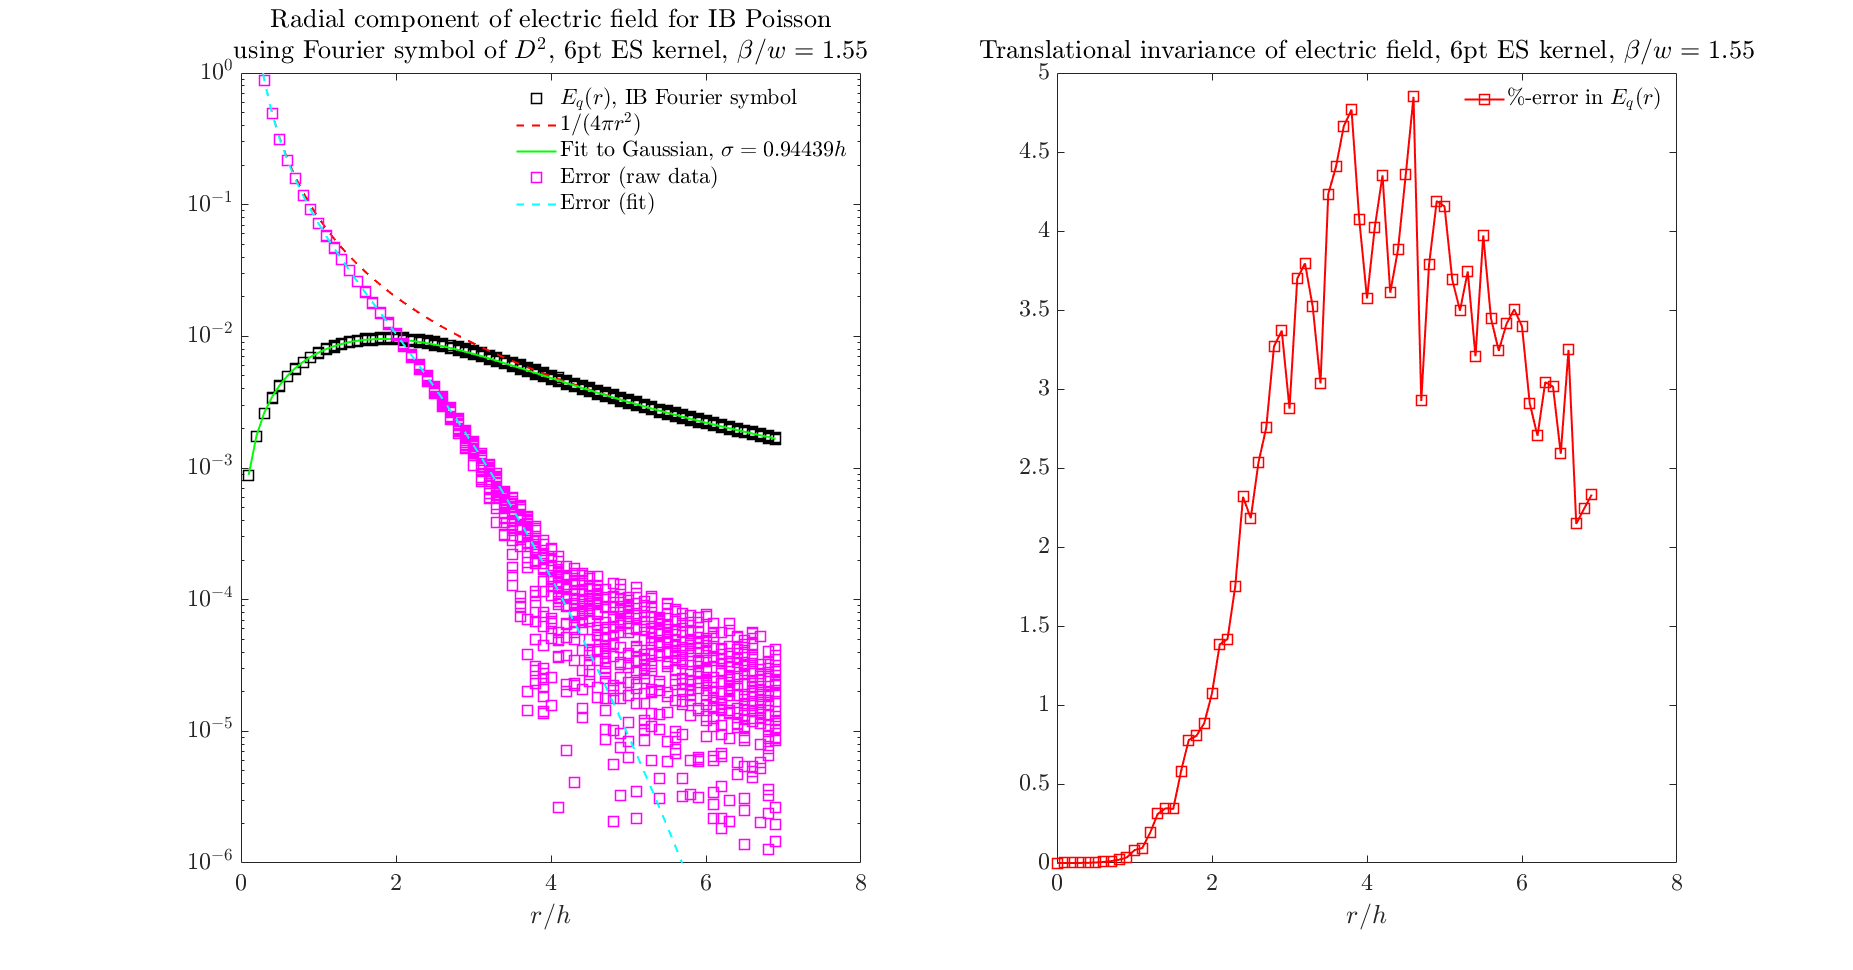
\includegraphics[width=1\columnwidth]{{../Figures/6pt_ES_beta1.55}.png}
	\caption{Results for 6pt ES kernel with $\beta/w = 1.55$.}\label{ES6}
\end{figure}

\begin{figure}[H]
	\centering
	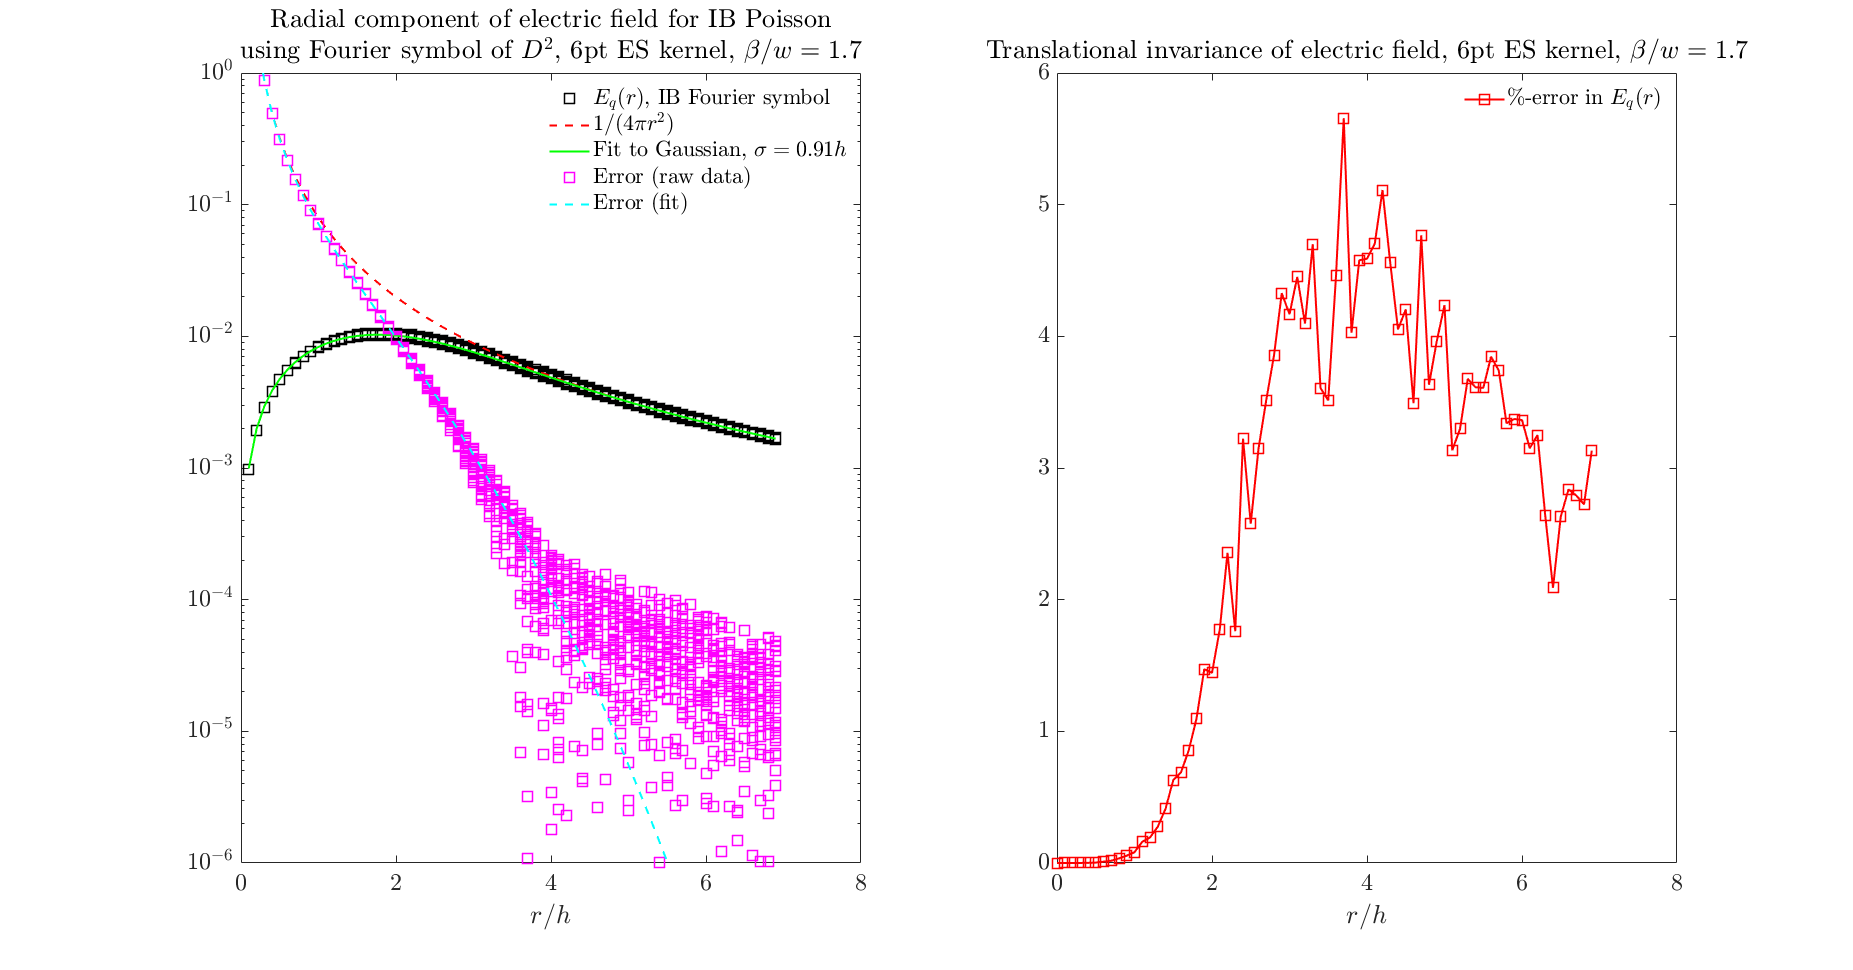
\includegraphics[width=1\columnwidth]{{../Figures/6pt_ES_beta1.7}.png}
	\caption{Results for 6pt ES kernel with $\beta/w = 1.7$.}\label{ES61}
\end{figure}

\begin{figure}[H]
	\centering
	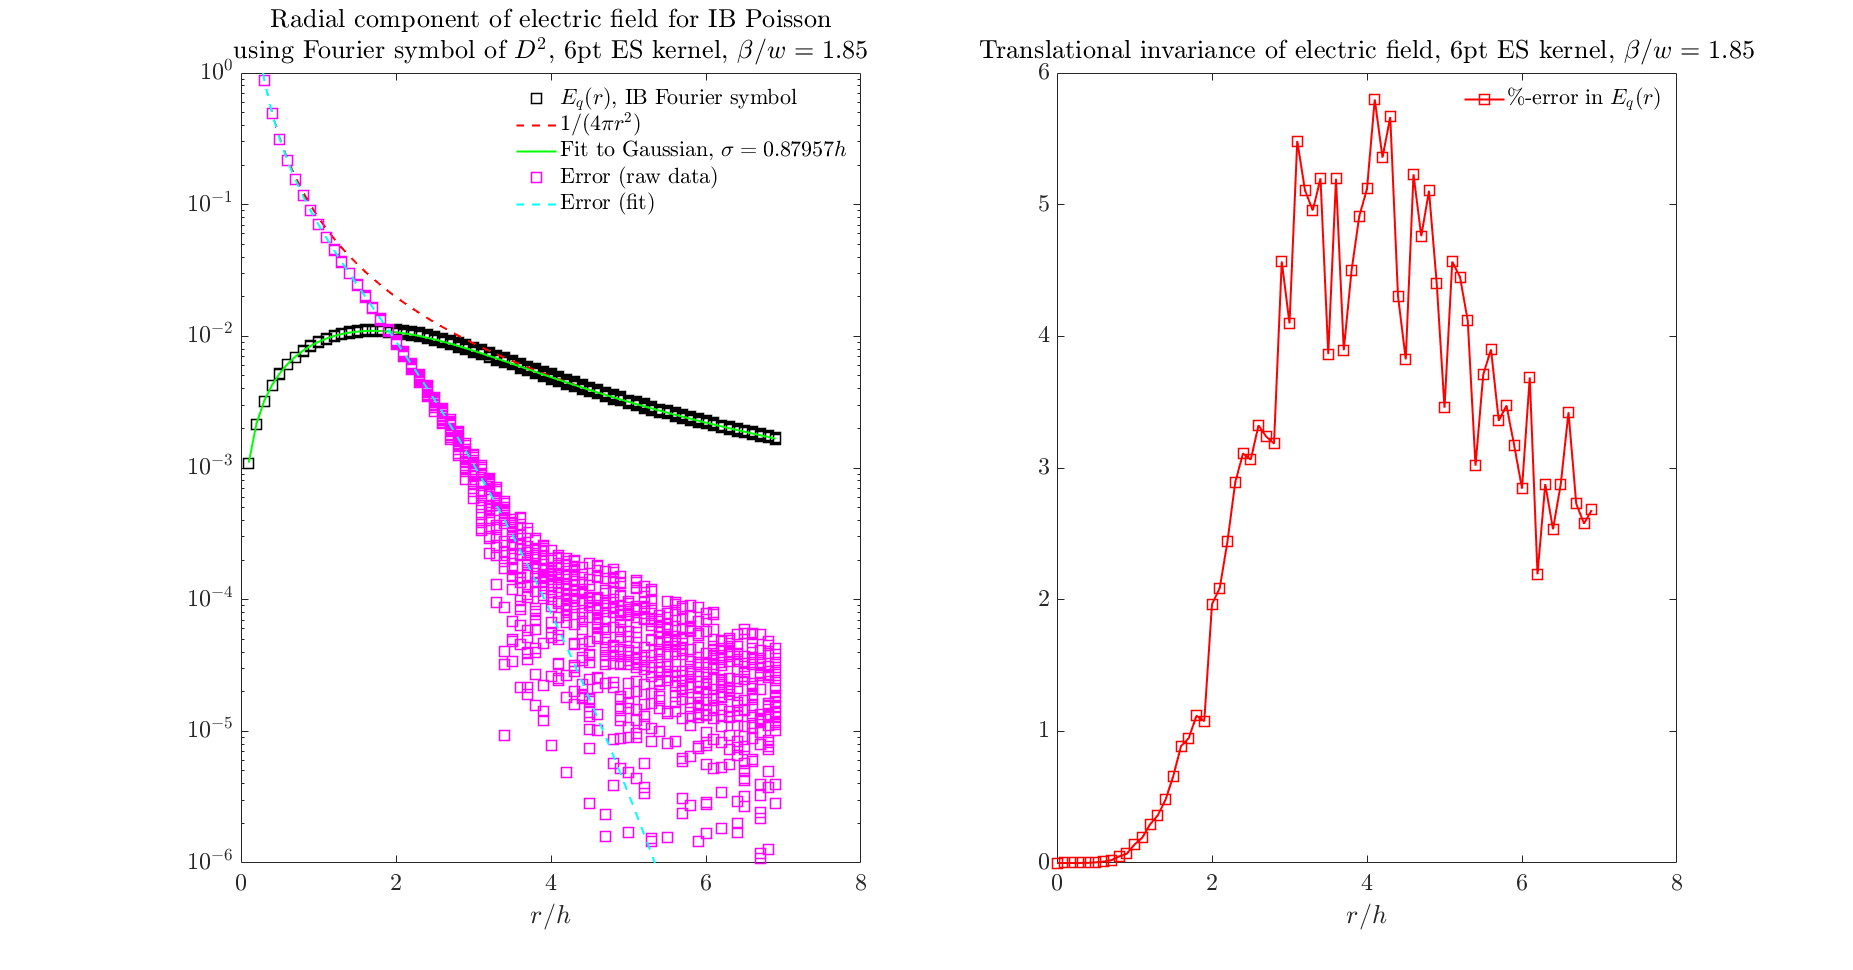
\includegraphics[width=1\columnwidth]{{../Figures/6pt_ES_beta1.85}.png}
	\caption{Results for 6pt ES kernel with $\beta/w = 1.85$.}\label{ES62}
\end{figure}

In the next figure, we use the spectral solver with $w=  6, \beta/w = 1.5,1.8,2.1$ to compare the loss in invariance between the finite-difference and spectral solvers.
\begin{figure}[H]
	\centering
	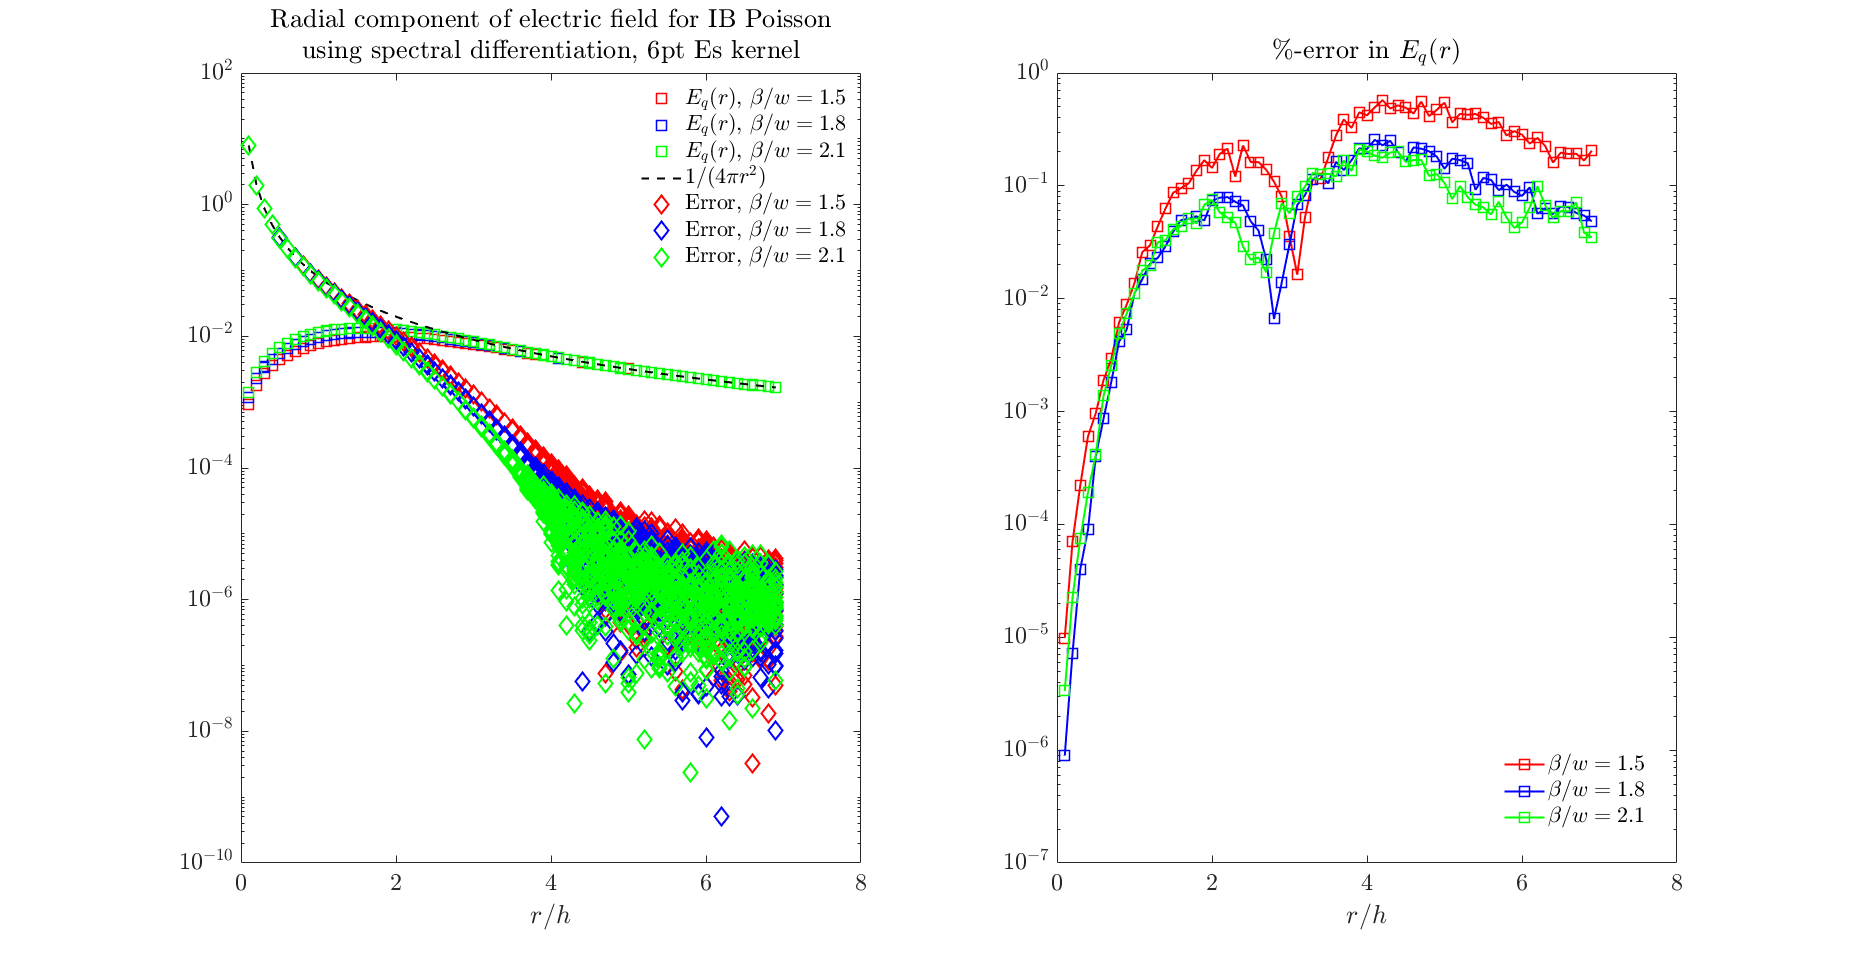
\includegraphics[width=1\columnwidth]{{../Figures/6pt_ES_spectral_beta1.5_1.8_2.1}.png}
	\caption{Results for 6pt ES kernel with $\beta/w = 1.5, 1.8,2.1$ using the spectral solver. Comparing this with the previous figures, it appears that we loose an order of magnitude in the invariance when using the finite-difference solver.}\label{ES63}
\end{figure}

\myssection{Non-central component of the electric field for each kernel}{}

\begin{figure}[H]
	\centering
	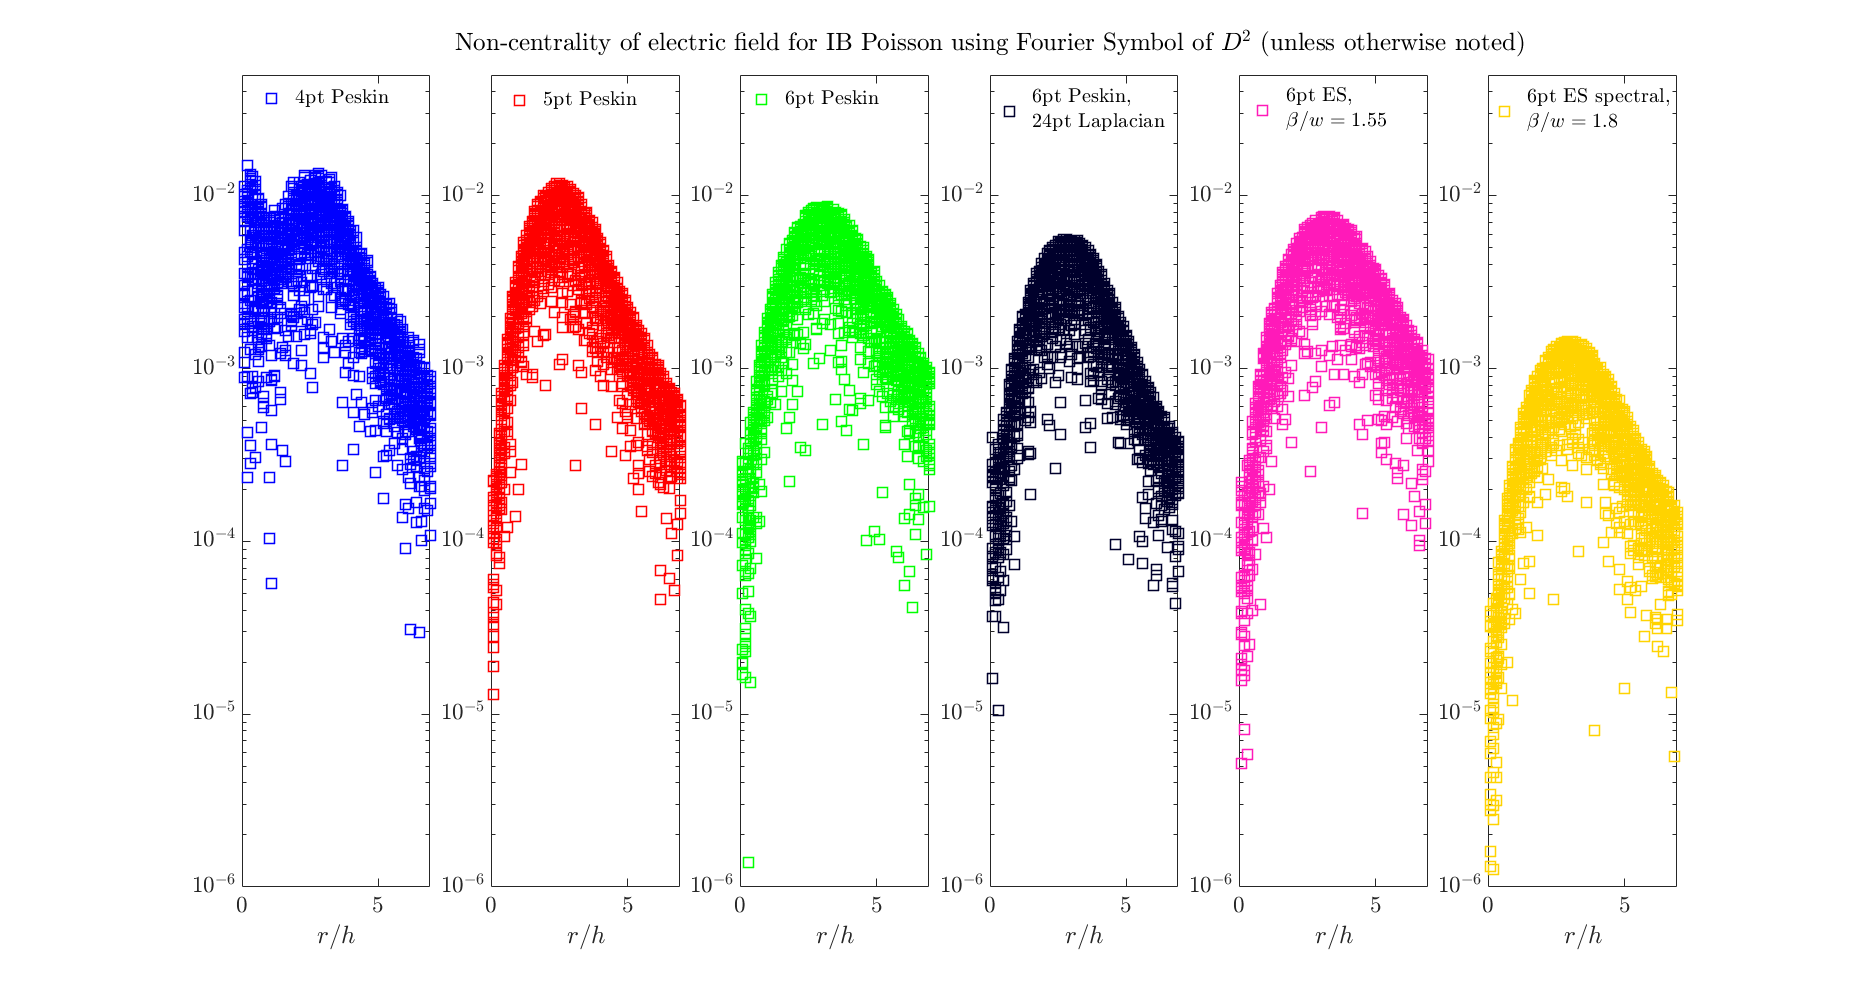
\includegraphics[width=1\columnwidth]{../Figures/nonC_all_new.png}
	\caption{Spread of non-central component of electric field for each kernel considered.}\label{nonC}
\end{figure}
\end{document}
